% Compile with XeLaTeX, TeXLive 2013 or more recent
\documentclass{beamer}

% Base packages
\usepackage{fontspec}
\usepackage{xunicode}
\usepackage{xltxtra}

\usepackage{amsfonts}
\usepackage{amsmath}
\usepackage{longtable}
\usepackage{csquotes}
\usepackage{standalone}

\usepackage{graphicx}
\graphicspath{{./images/}}

\usepackage{listings}
\lstset{basicstyle=\footnotesize\ttfamily, breaklines=true, keepspaces=true }

% Setup Russian hyphenation
\usepackage{polyglossia}
\setdefaultlanguage[spelling=modern]{russian} % for polyglossia
\setotherlanguage{english} % for polyglossia
\defaultfontfeatures{Scale=MatchLowercase, Mapping=tex-text}

% Setup fonts
\newfontfamily\russianfont{CMU Serif}
\setromanfont{CMU Serif}
\setsansfont{CMU Sans Serif}
\setmonofont{CMU Typewriter Text}

% Be able to insert hyperlinks
\usepackage{hyperref}
\hypersetup{colorlinks=true, linkcolor=black, filecolor=black, citecolor=black, urlcolor=blue , pdfauthor=Evgeny Yulyugin <yulyugin@gmail.com>, pdftitle=Параллельное программирование}
% \usepackage{url}

% Misc optional packages
\usepackage{underscore}
\usepackage{amsthm}

% A new command to mark not done places
\newcommand{\todo}[1][]{{\color{red}TODO\ #1}}

\newcommand{\abbr}{\textit{англ.}\ }

\subtitle{Курс «Параллельное программирование»}
\subject{Lecture}
\author[Евгений Юлюгин]{Евгений Юлюгин \\ \small{\href{mailto:yulyugin@gmail.com}{yulyugin@gmail.com}}}
\date{\today}
\pgfdeclareimage[height=0.5cm]{mipt-logo}{../common-images/mipt.png}
\logo{\pgfuseimage{mipt-logo}}

\typeout{Copyright 2014 Evgeny Yulyugin}

\usetheme{Berlin}
\setbeamertemplate{navigation symbols}{}%remove navigation symbols

\title{Title}

\begin{document}

\begin{frame}
\titlepage
\end{frame}

\section{Обзор}

\begin{frame}
\tableofcontents
\end{frame} 

\begin{frame}{На прошлой лекции}

\begin{itemize}
    \item Основы MPI.
\end{itemize}

\end{frame}

\section{Классификация архитектур вычислительных систем}

\begin{frame}{Классификация Флинна}

\begin{table}[htp]
    \begin{center}
    \begin{tabular}{|l|c|c|}
        \hline
                                & Single data   & Multiple data \\
        \hline
        Single instruction      & SISD          & SIMD \\
        \hline
        Multiple instruction    & MISD          & MIMD \\
        \hline
    \end{tabular}
    \end{center}
\end{table}

\end{frame}

\begin{frame}{Симметричная мультипроцессорность}

Симметричная мультипроцессорность (\abbr Symmetric Multiprocessing, MPP) --- архитектура вычислительных систем, в которой все процессоры подключаются к общей памяти (при помощи шины или подобного устройства) симметрично и имеют к ней однородный доступ.

Так же известна как UMA (Uniform Memory Access или Uniform Memory Architecture).

\end{frame}

\begin{frame}{Симметричная мультипроцессорность}

\begin{figure}[htp]
	\centering
	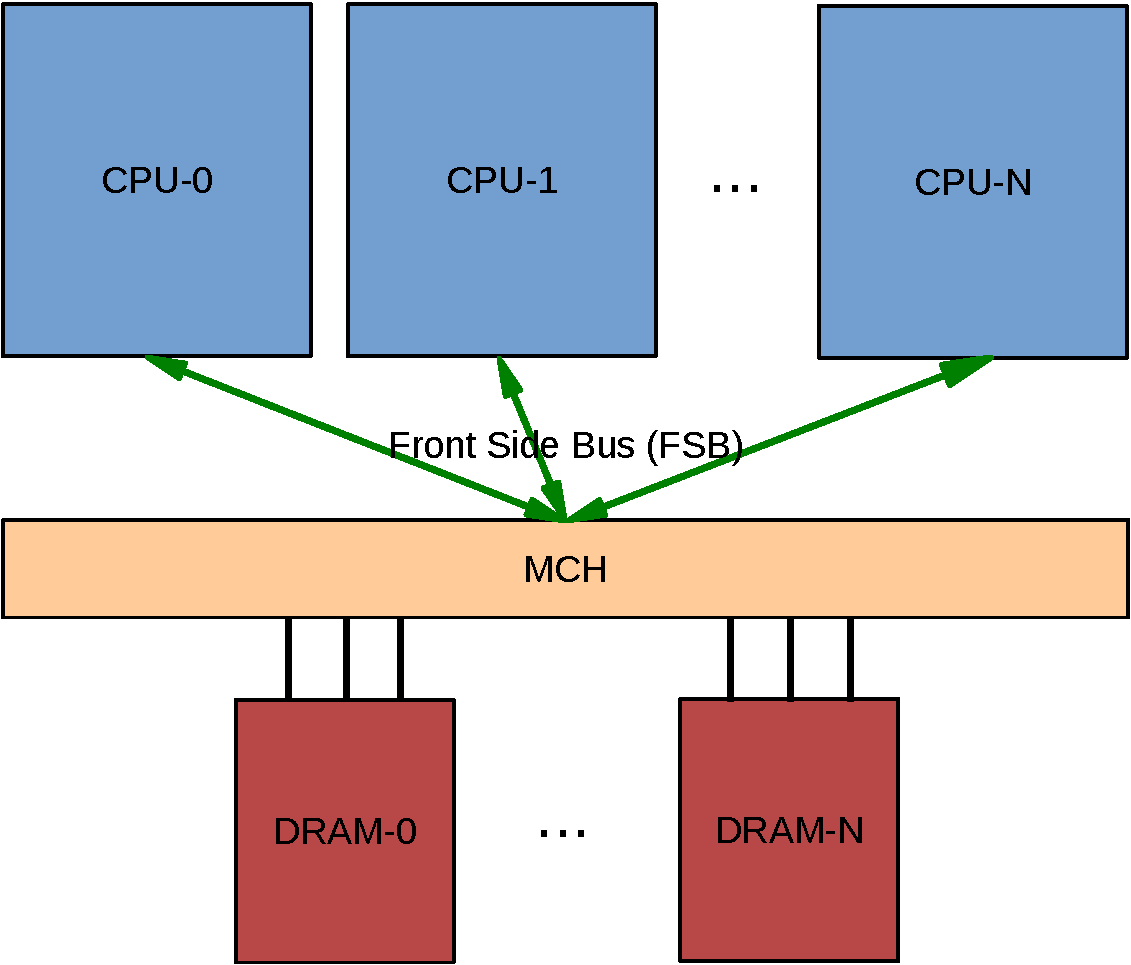
\includegraphics[width=0.7\textwidth]{SMP}
\end{figure}

\end{frame}

\begin{frame}{Массово-параллельная архитектура}

Массово-параллельная архитектура (\abbr Massive parallel processing, MPP) --- класс архитектур, в которых процессоры имеют доступ исключительно к локальным ресурсам. То есть память разделена физически.

\end{frame}

\begin{frame}{Массово-параллельная архитектура}

\todo Add a picture.

\end{frame}

\begin{frame}{Архитектура с неравномерной памятью}

NUMA (Non-Uniform Memory Access или Non-Uniform Memory Architecture) система разделяется на множественные узлы, имеющие доступ как к своей локальной памяти, так и к памяти других узлов.

\end{frame}

\begin{frame}{Архитектура с неравномерной памятью}

\todo Add a picture.

\end{frame}

\section{Состояние гонки}

\begin{frame}{Определение}

Состояние гонки (\abbr Race condition) --- ошибка в многопоточной программе, при которой работа приложения зависит от того, в каком порядке выполняются части кода.

Свое название получила от похожей ошибки проектирования электронных схем (Гонки сигналов).

Состояние гонки --- ошибка проявляющаяся в случайный момент времени.

\end{frame}

\begin{frame}[fragile]{Пример}

\begin{lstlisting}[language=C++,basicstyle=\ttfamily,keywordstyle=\color{blue},basicstyle=\scriptsize]
int N = 1000;
int x = 0;
\end{lstlisting}

\begin{columns}[t]
    \begin{column}[T]{0.45\textwidth}
    \begin{lstlisting}[language=C++,basicstyle=\ttfamily,keywordstyle=\color{blue},basicstyle=\scriptsize]
// thread 0
for (i = 0; i < N; ++i) {
    ++x;
}
    \end{lstlisting}
    \end{column}
    \begin{column}[T]{0.45\textwidth}
    \begin{lstlisting}[language=C++,basicstyle=\ttfamily,keywordstyle=\color{blue},basicstyle=\scriptsize]
// thread 1
for (i = 0; i < N; ++i) {
    if (x%2 == 0)
        printf("%d\n", x%2);
}
    \end{lstlisting}
    \end{column}
\end{columns}

\end{frame}

\section{Синхронизация}

\begin{frame}{Семафор}

Семафор --- объект, ограничивающий количество потоков, которые могут войти в заданный участок кода.

Интерфейс семафора:

\begin{itemize}
    \item init(n) --- установить счетчик в n,
    \item enter() --- подождать пока счетчик не станет больше нуля, затем уменьшить его на единицу,
    \item leave() --- увеличить счетчик на еденицу.
\end{itemize}

\end{frame}

\begin{frame}{Мьютекс}

Мьютекс (\abbr mutex) --- <<одноместный>> семафор, служащий для синхранизации одновременно выполняющихся потоков.

\todo Mutex types.

\end{frame}

\begin{frame}[fragile]{Взаимная блокировка}

Взаимная блокировка (\abbr deadlock) --- ситуация в многозадачной среде, при которой несколько процессов находятся в состоянии бесконечного ожидания ресурсов, занятых самими этими процессами.

\vfill

\begin{lstlisting}[language=C++,basicstyle=\ttfamily,keywordstyle=\color{blue},basicstyle=\footnotesize]
pthread_mutex_t A, B;
pthread_mutex_init(&A, NULL);
pthread_mutex_init(&B, NULL);
\end{lstlisting}

\begin{columns}[t]
    \begin{column}[T]{0.45\textwidth}
        \begin{lstlisting}[language=C++,basicstyle=\ttfamily,keywordstyle=\color{blue},basicstyle=\scriptsize]
// thread 0
pthread_mutex_lock(&A);
pthread_mutex_lock(&B);
// ...
        \end{lstlisting}
    \end{column}
    \begin{column}[T]{0.45\textwidth}
        \begin{lstlisting}[language=C++,basicstyle=\ttfamily,keywordstyle=\color{blue},basicstyle=\scriptsize]
// thread 1
pthread_mutex_lock(&B);
pthread_mutex_lock(&A);
// ...
        \end{lstlisting}
    \end{column}
\end{columns}

\end{frame}

\begin{frame}{Livelock}

Ситуация, когда в отличие от обычной блокировки процессы не зависают, а занимаются бесполезной работой.

Состояние системы постоянно меняется, но при этом она <<зациклилась>> и не производит полезной работы.

\end{frame}

\begin{frame}[fragile]{Алгоритм Деккера}

\begin{lstlisting}[language=C++,basicstyle=\ttfamily,keywordstyle=\color{blue},basicstyle=\scriptsize]
bool flag[2] = {false, false};
bool turn = false; // or true
\end{lstlisting}

\begin{columns}[t]
    \begin{column}[T]{0.45\textwidth}
        \begin{lstlisting}[language=C++,basicstyle=\ttfamily,keywordstyle=\color{blue},basicstyle=\scriptsize]
// thread 0
flag[0] = true;
while (flag[1]) {
    if (turn) {
        flag[0] = false;
        while (turn);
        flag[0] = true;
    }
}

// critical section
//...
turn = true;
flag[0] = false;
// end of critical section
// ...
        \end{lstlisting}
    \end{column}
    \begin{column}[T]{0.45\textwidth}
        \begin{lstlisting}[language=C++,basicstyle=\ttfamily,keywordstyle=\color{blue},basicstyle=\scriptsize]
// thread 1
flag[1] = true;
while (flag[0]) {
    if (!turn) {
        flag[1] = false;
        while (!turn);
        flag[1] = true;
    }
}

// critical section
//...
turn = false;
flag[0] = false;
// end of critical section
// ...
        \end{lstlisting}
    \end{column}
\end{columns}

\end{frame}

\section{Конец}
% The final "thank you" frame 

\begin{frame}{Задания}

Вычислить $\sum \limits_{n=0}^{N} \frac{1}{N!}$.

N --- аргумент командной строки.

Построить график времени работы в зависимости от количества процессов и ускорения в зависимости от количества процессов.

\end{frame}

\begin{frame}{На следующей лекции}
\end{frame}

\begin{frame}

{\huge{Спасибо за внимание!}\par}

\vfill

\tiny{\textit{Замечание}: все торговые марки и логотипы, использованные в данном материале, являются собственностью их владельцев. Представленная здесь точка зрения отражает личное мнение автора, не выступающего от лица какой-либо организации.}

\end{frame}

\end{document}
